\documentclass{standalone}
\usepackage{tikz}
\usetikzlibrary{calc}
\begin{document}
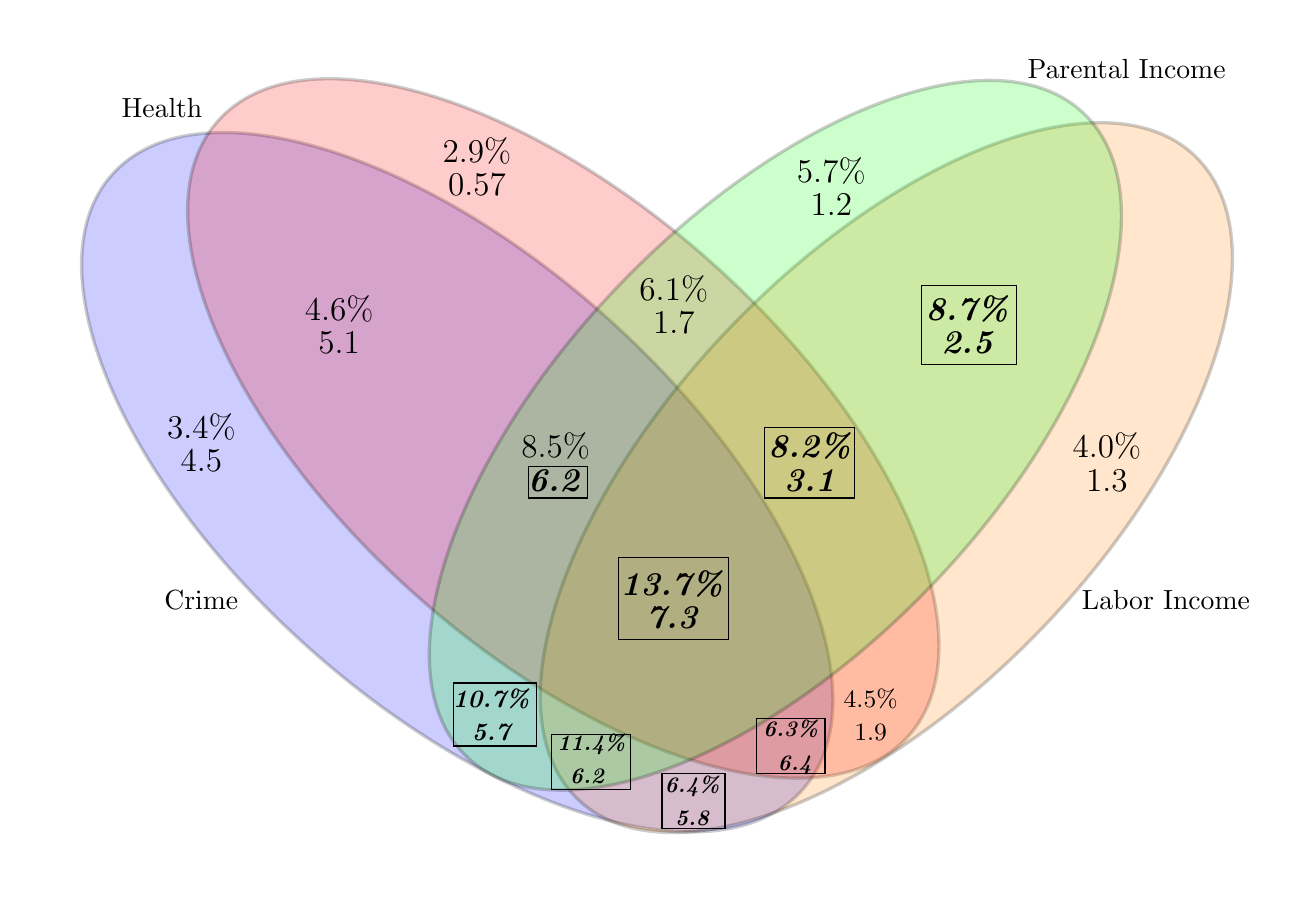
\begin{tikzpicture}

\begin{scope}[shift={(-2,0)},x={(2,2)},y={($(-2,0)!1!60:(2,2)$)}]
  \draw[black, very thick, fill=blue, opacity=.2] (.5,0) ellipse (1 and .5);
\end{scope}
\begin{scope}[shift={(-2,0)},x={(2,2)},y={($(-2,0)!1!60:(2,2)$)}]
  \draw[black, very thick, fill=red, opacity=.2] (1,-.04) ellipse (1 and .5);
\end{scope}

\begin{scope}[shift={(2,0)},x={(-2,-2)},y={($(2,0)!1!60:(-2,-2)$)}]
  \draw[black, very thick, fill=orange, opacity=.2] (-.9,-0.125) ellipse (2 and .35);
\end{scope}
\begin{scope}[shift={(2,0)},x={(-2,-2)},y={($(2,0)!1!60:(-2,-2)$)}]
  \draw[black, very thick, fill=green, opacity=.2] (-.65,.05) ellipse (2 and .35);
\end{scope}

\draw (-4.25,2) node[align=center, below] {\large 3.4\% \\ \large  4.5 }; 		%A
\draw (-0.75,5.5) node[align=center, below] {\large 2.9\% \\ \large 0.57 }; 						%B
\draw (3.75,5.25) node[align=center, below] {\large 5.7\% \\ \large 1.2  }; 				%C
\draw (7.25, 1.75) node[align=center, below] {\large 4.0\% \\  \large 1.3 }; 						%D
\draw (-2.5,3.5) node[align=center, below] {\large 4.6\% \\ \large 5.1 }; 						%AB
\draw (-.55,-1.5) node[align=center, below] {\small \textit{\textbf{10.7\%}} \\ \small \textit{\textbf{5.7}} }; 				%AC

\draw (2,-2.6) node[align=center, below] {\footnotesize \textit{\textbf{6.4\%}}  \\ \footnotesize  \textit{\textbf{5.8}} }; 						%AD
\draw (1.75,3.75) node[align=center, below] {\large 6.1\% \\ \large 1.7 }; 					%BC
\draw (4.25,-1.5) node[align=center, below] {\small 4.5\% \\ \small 1.9 }; 						%BD
\draw (5.5,3.5) node[align=center, below] {\large \textit{\textbf{8.7\%}}  \\ \large \textit{\textbf{2.5}}}; 			%CD
\draw (0.25, 1.75) node[align=center, below] {\large 8.5\% \\ \large \textit{\textbf{6.2}}  }; 					%ABC
\draw (3.25,-1.9) node[align=center, below] {\footnotesize \textit{\textbf{6.3\%}} \\ \footnotesize \textit{ \textbf{6.4}}}; 						%ABD
\draw (0.72,-2.07) node[align=center, below] {\footnotesize \textit{\textbf{11.4\%}} \\ \footnotesize \textit{\textbf{6.2} } }; 			%ACD
\draw (3.5, 1.75) node[align=center, below] {\large \textit{\textbf{8.2\%}} \\ \large \textit{\textbf{3.1}}}; 					%BCD
\draw (1.75,0) node[align=center, below] {\large \textit{\textbf{13.7\%}} \\ \large \textit{\textbf{7.3}} }; 		
\draw (.65,1.2) rectangle (-.1,0.8);											%ABCD
\draw (1.05,-1) rectangle (2.45,.04);
\draw (2.9,1.7) rectangle (4.05,.8);
\draw (4.9,2.5) rectangle (6.1,3.5);
\draw (-1.05,-1.55) rectangle (0.01,-2.35);
\draw (0.2,-2.9) rectangle (1.2,-2.2);
\draw (1.6,-3.4) rectangle (2.4,-2.7);
\draw (2.8,-2.7) rectangle (3.67,-2);

\draw [black] (-4.25,-.25) node[align=center, below] {Crime};
\draw [black] (-4.75,6) node[align=center, below] {Health};

\draw [black] (8,-.25) node[align=center, below] {Labor Income};
\draw [black] (7.5,6.5) node[align=center, below] {Parental Income};



\end{tikzpicture}
\end{document}


